% Chapter 11 (English edition) -- ED-20: the triangular lattice is not a local minimum of the zero-point energy for exp(-pi r^2)
% Translated from papers/discovery_journal_2026/chapters/c11.tex. Figure: code/fig11.py.
\chapter{Perfect at rest, not when it trembles}

\reference{Published on 26 October 2026. doi:10.5281/zenodo.23655392}

\section*{The idea in one picture}

Picture marbles that push each other away, lying on a table. Left alone, they settle into
triangles: each marble has six neighbours, like the cells of a honeycomb. For the force studied
here, a bell-shaped repulsion (it equals $e^{-\pi r^2}$ at distance $r$), this triangular
arrangement is the best of the regular lattices when the marbles are motionless. That is an old
result from the literature, which this work quotes second-hand and does not re-check.

But in quantum physics nothing is ever completely still. Even at absolute zero, every particle
trembles a little, and this trembling costs an energy called the ``zero-point energy''. The
question, labelled QU-1 in the project, was a natural one: does the lattice that wins at rest
also win once this trembling is counted? An earlier approximate calculation (pencil-and-paper
in spirit, level~X) already said no. This chapter tells how that ``no'' was made certain, on
one precise piece of the question.

\begin{analogie}
You believed the marble was sitting at the bottom of a bowl. You nudge it by a hair, in a
well-chosen direction, and find that the height goes down: so it was not the bottom after all.
\emph{Where the picture stops:} here nothing rolls; we compare the energies of two frozen
arrangements, very close to each other. And from this result alone we cannot tell whether we
were on top of a bump or on a saddle: we only know that it was not the bottom.
\end{analogie}

\section*{What was done}

We start from the triangular lattice and deform it by an amount $t$, with a slight shear that
keeps the same area per marble. Write $E(t)$ for the zero-point energy per marble. The work
shows that $E(t)<E(0)$ for every non-zero $t$ with $|t|\le 10^{-5}$.

The energy $E(t)$ is an average of square roots of matrices, which is very hard to pin down
directly. The trick is to build a \emph{roof} $U(t)$: a function that always lies above $E$ and
touches it exactly at $t=0$. If the roof goes down on both sides of $0$, the ground beneath it
goes down too. For this it is enough to prove that the curvature of the roof stays negative over
the whole small window; the certified computation bounds it by $-1.84156$. Then
$E(t)-E(0)\le -0.92\,t^2$: at $t=10^{-5}$, a drop of at least $9\times10^{-11}$ in the units of
the computation. It is tiny, but it is a certain sign.

\begin{encadre}
\textbf{To do with a pencil: why the roof lies above.} Take a number $d$ and a guess $x$ for its
square root. Since $(\sqrt d - x)^2\ge 0$, we always have
\[\sqrt d\;\le\;\tfrac12\Bigl(x+\frac{d}{x}\Bigr),\]
with equality when $x=\sqrt d$. Try $d=10$, $x=3$: the right-hand side is
$\tfrac12(3+\tfrac{10}{3})=\tfrac{19}{6}\approx3.1667$, and $\sqrt{10}\approx3.1623$ is indeed
below it. The work uses the same inequality for $2\times2$ matrices.

\textbf{To do with a pencil: the final sign.} The three certified numbers, rounded here
against ourselves (toward the side that brings us closer to zero), are $-1.900167$,
$1.833534$ and $0.031965$. The bound is at most
$-1.900167+1.833534\times0.031965\approx-1.900167+0.058609=-1.841558$,
which is negative. The Lean program redoes this computation with exact fractions.
\end{encadre}

\section*{How we made sure it is not wrong}

The chain has three links, and they are not of the same level.
\niveau{A} \emph{The judge has looked} for the logic and the arithmetic: the inequality for
$2\times2$ matrices, the reasoning ``the roof goes down, so the ground goes down'', and the sign
of the fractions are checked step by step by the Lean kernel, the small program that judges
proofs. The axioms stay within the short allowed list, and a replay of the module by the kernel
passed.
\niveau{C} for the integrals, in the sense that nobody has checked them by machine: they are
enclosed by rigorous interval arithmetic (206,468 cells, none failing), run by a program but not
re-read by the judge. \niveau{C} also for the ``glue'': a piece of reasoning, carried out here
by AI agents and not by a human, that neither a machine nor a person has verified. The overall
result is therefore level~C, and the paper says so.

The controls did their job. For a narrower bell ($e^{-2\pi r^2}$), the triangular lattice
\emph{is} a local minimum according to the approximate calculation: the same method must then
fail, and it does fail (the bound stays positive, around $+12.8$), and the judge rejects the
certificate. A false proof planted on purpose is exposed by the list of axioms. A separate
auditor agent redid the computation with cells 8 to 25 times wider: the sign stays negative. It
also recoded the quantities another way, in floating-point arithmetic, and found values inside
the enclosures. Its verdict, ``accept with corrections'', asked for two text corrections,
including one false mathematical sentence; both have been applied. No human has read this work.

\section*{What this does not say}

\begin{limite}
\begin{itemize}
\item A single path of deformation, a window of $10^{-5}$, a single force, regular lattices in
  two dimensions, and the ``harmonic'' approximation of the vibrations.
\item The result goes one way only: the method can say ``not a minimum'', never ``minimum''. It
  bounds a curvature from above, without enclosing it on both sides.
\item The goal announced in advance (a curvature certified on both sides) was not reached; the
  paper flags this as a departure from the preregistration.
\item The same certificate works for $e^{-\pi r^2/2}$, but that case was not planned: it is a
  by-product, not a test.
\item Nothing is said about the best lattice for the zero-point energy, nor about the full
  quantum crystal.
\end{itemize}
\end{limite}

It is a useful lesson all the same: ``the best at rest'' and ``the best when trembling'' do not
coincide, and we now know it beyond the approximate calculation.

\section*{Going further}

The paper (8 pages) gives the proof step by step, next to the corresponding Lean statements:
doi:10.5281/\allowbreak zenodo.23655392. The same question, for more physical forces, is taken up
in doi:10.5281/\allowbreak zenodo.23663551.

\begin{figure}[ht]
\centering
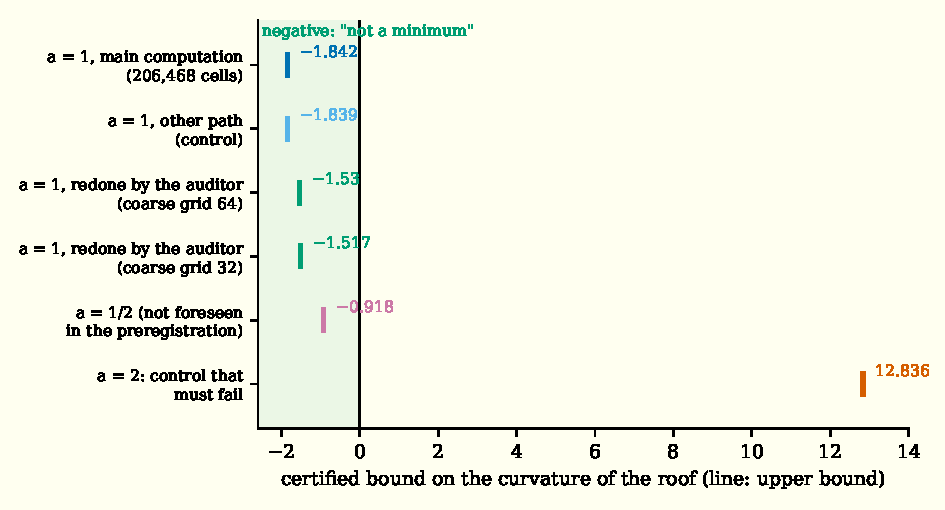
\includegraphics[width=\linewidth]{figures/c11_courbures}
\caption{Certified curvature bounds: negative for $a=1$ (computation, control, the auditor's redos) and for $a=1/2$, positive for the control $a=2$.}
\end{figure}
